\title{Casper the Friendly Finality Gadget}
\author{
        Vitalik Buterin \\
        Ethereum Foundation}


\documentclass[12pt, final]{article}

%% make in the latest NIPS format (as of this writing, 2017)

\usepackage[nonatbib,final]{nips_2017}
%\usepackage[nonatbib,final]{nips_2017}

\usepackage{color}
\usepackage{graphicx}
\DeclareGraphicsExtensions{.pdf,.eps,.png,.jpg}     % search for .pdf, then .eps, then .pngs, then .jpg

% look in these subdirectories for graphics referenced by \includegraphics
% each entry must end with a /
\graphicspath{{figs/}{figures/}{images/}{./}}

\newcommand*{\red}[1]{ \color{red} #1}

%\usepackage{tabularx}
\usepackage{url}
\usepackage{amsmath}

% this is for environments \subfigure and \subtable
\usepackage{subcaption}

% These packages are FORBIDDEN
%%%%%%%%%%%%%%%%%%%%%%%%%%%%%%%%%%%%%%%%%%%%%%%%%%%%%%%%
%\usepackage{lmodern} % messes up \textsc
%\usepackage{cite} % messes up NIPS
%\usepackage{fullpage} % messes up NIPS
%\usepackage{natbib} % messes up NIPS
%%%%%%%%%%%%%%%%%%%%%%%%%%%%%%%%%%%%%%%%%%%%%%%%%%%%%%%%

\usepackage{array}          % replacement for eqnarray.  Must be BEFORE \usepackage{arydshln}
\usepackage{units}          % for \nicefrac{\alpha}{\beta}


\usepackage{amsthm}     % for theorems
\newtheorem{definition}{Definition}

% text looks a little better
\usepackage{microtype}

\usepackage{wasysym}

\usepackage{textcomp, marvosym} % pretty symbols
\usepackage{booktabs}   % for much better looking tables

% for indicator functions
\usepackage{dsfont}

% For automatic capitalizaton of section names, etc.
\usepackage{titlesec,titlecaps}


\Addlcwords{is with of the and in}
\Addlcwords{of the}
\Addlcwords{and}
\titleformat{\section}[block]{}{\normalfont\Large\bfseries\thesection.\;}{0pt}{\formatsectiontitle}
\newcommand{\formatsectiontitle}[1]{\normalfont\Large\bfseries\titlecap{#1}}

\titleformat{\subsection}[block]{}{\normalfont\large\bfseries\thesubsection.\;}{0pt}{\formatsubsectiontitle}
\newcommand{\formatsubsectiontitle}[1]{\normalfont\large\bfseries\titlecap{#1}}





% for pretty Euler script
% \usepackage[mathscr]{euscript}
% \usepackage{bold-extra}





%\usepackage{subfig}
\usepackage{float} % for \subfloat

%%%%%%%%%%%%%%%%%%%%%%%%%%%%%%%%%%%%%%%%%%
%% More customizable Lists
%%%%%%%%%%%%%%%%%%%%%%%%%%%%%%%%%%%%%%%%%%
% Better symbols custom enumerative lists, define any symbol you'd like
% \usepackage{enumitem}


%%%%%%%%%%%%%%%%%%%%%%%%%%%%%%%%%%%%%%%%%%
%% Custom Symbols 
%%%%%%%%%%%%%%%%%%%%%%%%%%%%%%%%%%%%%%%%%%
% \xspace at the end of custom macros never screws up spacing.
\usepackage{xspace}



%%%%%%%%%%%%%%%%%%%%%%%%%%%%%%%%%%%%%%%%
%% Abbreviations you'll always want
%%%%%%%%%%%%%%%%%%%%%%%%%%%%%%%%%%%%%%%%
\newcommand*{\TODO}[1]{{\centering {\small \sffamily \color{red} #1} \vskip10pt }}
\newcommand*{\todo}[1]{{\small \sffamily [{\color{red} #1}]}}
\newcommand*{\q}[1]{{\small \sffamily [{\color{blue} #1}]}}
\newcommand*{\fix}[1]{{\sffamily [{\textnormal{\color{red} #1}}]}}



%-----------------------------------------------------------------------------
%  Cross references
%-----------------------------------------------------------------------------
% The following code defines how you make references to figures, tables, etc...
% It is defined in one place only, and can be modified for all references
% in the document at the same time.
% Instead of typing each time: "see Fig. \ref{myfig}" you can create a command
% \figref which will do the job. Then in text you only type \figref{myfig} and LaTeX
% will do the rest.
\newcommand{\tblref}[1]{Table~\ref{#1}}
%\renewcommand*{\figref}[1]{Fig.~\ref{#1}}
\renewcommand{\eqref}[1]{eq.~(\ref{#1})}
\newcommand{\Subref}[1]{(\subref{#1})}


\newcommand{\figref}[1]{Figure~\ref{#1}}
\newcommand{\Figref}[1]{Figure~\ref{#1}}
\newtheorem{theorem}{Theorem}
\newtheorem{lemma}[theorem]{Lemma}

%%%%%%%%%%%%%%%%%%%%%%%%%%%%%%%%%%%%%%%%

% for \sout{} for strikeout
% \usepackage[normalem]{ulem}


% for better manipulation of tables
\usepackage{makecell}
\renewcommand\theadfont{\bfseries}


%-----------------------------------------------------------------------------
%  Misc symbols that I like
%-----------------------------------------------------------------------------
\newcommand*{\opname}[1]{\operatorname{#1}}


\renewcommand*{\to}{\rightarrow}


%%%%







\usepackage{color}
\newcommand*{\todo}[1]{\color{red} #1}
\newcommand{\eqref}[1]{eq.~\ref{#1}}
\newcommand{\figref}[1]{Figure~\ref{#1}}
\usepackage{amsthm}
\newtheorem{theorem}{Theorem}
\usepackage{graphicx}
\graphicspath{{figs/}{figures/}{images/}{./}}

%% Special symbols we'll probably iterate on
%%%%%%%%%%%%%%%%%%%%%%%%%%%%%%%%%%%%%%%%%%%%%%%%%%%%%%
% we will probably iterate on these symbols until we have a notation we like
\newcommand{\epoch}{\ensuremath{e}\space}
\newcommand{\hash}{\textnormal{h}\space}

% symbols for the epoch and hash source
\newcommand{\epochsource}{\ensuremath{\epoch_{\star}}\space}
\newcommand{\hashsource}{\ensuremath{\hash_{\star}}\space}

\newcommand{\signature}{\ensuremath{\mathcal{S}}\space}

\newcommand{\totaldeposit}{\textnormal{TD}\space}

\newcommand{\gamesymbol}{\reflectbox{G}}

\newcommand{\msgPREPARE}{\textbf{\textsc{prepare}}\space}
\newcommand{\msgCOMMIT}{\textbf{\textsc{commit}}\space}

% Symbols for the Last Justified Epoch and Hash
\newcommand{\epochLJ}{\ensuremath{\epoch_{\textnormal{LJ}}}\space}
\newcommand{\hashLJ}{\ensuremath{\hash_{\textnormal{LJ}}}\space}

% Symbols for the Last Finalized Epoch and Hash
\newcommand{\epochLF}{\ensuremath{\epoch_{\textnormal{LF}}}\space}
\newcommand{\hashLF}{\ensuremath{\hash_{\textnormal{LF}}}\space}

% Griefing Factor symbol
\newcommand{\GF}[1]{\mathds{GF}\left( #1 \right)\space}

% Genesis block symbol
\newcommand{\Genesisblock}{\ensuremath{G}\space}

\begin{document}

\maketitle

\begin{abstract}
We give an introduction to the consensus algorithm details of Casper: the Friendly Finality Gadget, as an overlay on an existing proof of work blockchain such as Ethereum. Casper is a partial consensus mechanism inspired by a combination of existing proof of stake algorithm research and Byzantine fault tolerant consensus theory, which if overlaid onto another blockchain (which could theoretically be proof of work or proof of stake) adds strong \textit{finality} guarantees that improve the blockchain's resistance to transaction reversion (or ``double spend'') attacks.
\end{abstract}

\section{Introduction}
\label{sect:intro}

Over the past few years there has been considerable research into ``proof of stake''-based blockchain consensus algorithms. In a proof of stake system, a blockchain grows and agrees on new blocks through a process where anyone who holds coins inside of the system can participate, and the amount of influence that any given coin holder has is proportional to the number of coins (or ``stake'') that they hold. This represents an alternative to proof of work ``mining'', allowing blockchains to operate without the high hardware and electricity costs that proof of work blockhains require.

There have been two major schools of thought in proof of stake algorithm design. The earlier of the two, \textit{chain-based proof of stake}, tries to closely mirror the mechanics of proof of work, featuring a chain of blocks and an algorithm that ``simulates'' mining by pseudorandomly assigning the right to create new blocks to stakeholders. This includes Peercoin\cite{king2012ppcoin}, Blackcoin\cite{vasin2014blackcoin} and Iddo Bentov's work\cite{bentov2016pos}.

The other school, \textit{BFT-based proof of stake}, is based on a thirty year old body of research into \textit{Byzantine fault tolerant consensus algorithms} such as PBFT \cite{castro1999practical}. BFT algorithms tend to have strong and rigorously proven mathematical properties; for example, one can usually mathematically prove that as long as at more than $\frac{2}{3}$ of participants in the protocol are following the protocol correctly, then the algorithm cannot possibly finalize conflicting block hashes at the same time (``safety''); this result holds regardless of network latency. The suggestion of repurposing BFT algorithms for proof of stake was first introduced by Tendermint\cite{kwon2014tendermint}.

\subsection{Our Work}

We present an algorithm that follows in the latter tradition, though with some modifications. Casper the Friendly Finality Gadget takes the form of an \textit{overlay} on top of some kind of \textit{proposal mechanism} - a mechanism which proposes \textit{checkpoints} which the Casper mechanism can then set in stone by \textit{finalizing} them.  Casper depends on the proposal mechanism for liveness, but not safety; that is, if the proposal mechanism is entirely controlled by attackers, then the attackers can prevent Casper from finalizing any future checkpoints, but cannot cause a safety failure in Casper---i.e., they cannot force Casper to finalize two conflicting blocks.

The proposal mechanism will initially be the existing Ethereum proof of work chain, making the first version of Casper a \textit{hybrid PoW/PoS algorithm} that relies on proof of work for liveness but not safety, but in future versions the proposal mechanism can be substituted with something else.

Our algorithm introduces several new properties that BFT algorithms by themselves do not necessarily support. First, we change the emphasis of the proof statement from the traditional ``as long as more than $\frac{2}{3}$ of validators are honest, there will be no safety failures'' to the contrapositive ``if there is a safety failure, that implies that $\ge \frac{1}{3}$ of validators violated some protocol rule'', and furthermore we add \textit{accountability}: ``$\ge \frac{1}{3}$ violated the rules, \textit{and we know who they are}''.

Accountability allows us to penalize malfeasant validators, solving the \textit{nothing at stake} problem that often plagues chain-based proof of stake algorithms. The size of the penalty is equal to the size of validators' entire deposits; this ensures that the cost of violating protocol guarantees is much higher than the size of the rewards that the system pays out during normal operation, achieving a much \textit{stronger} security guarantee than is possible with proof of work.

Second, the design of the algorithm as an overlay makes it easier to implement as an upgrade to a proof of work base chain. Third, we introduce a provably safe way of allowing the validator set to change over time. Finally, we introduce a way to recover from attacks where more than $\frac{1}{3}$ of validators drop offline, at the cost of a very weak \textit{tradeoff synchronicity assumption}.

\section{The Protocol}
\label{sect:protocol}

We will describe the protocol in stages, starting with a simple version and then progressively adding features such as validator set changes and mass liveness fault recovery. In the simple version, we simply assume that there is a set of validators, as well as a \textit{proposal mechanism} which is either a proof of work chain or something which exhibits similar behavior. We define an \textit{epoch} as a range of 100 blocks (e.g. blocks 600...699 are epoch 6), and a \textit{checkpoint} as the hash of a block right before the start of an epoch. The \textit{epoch of a checkpoint} is the epoch \textit{after} the checkpoint, e.g. the epoch of a checkpoint which is the hash of some block 599 is 6. Validators have the ability to make two types of messages:

$$\langle \msgPREPARE, \hash, \epoch, \hashsource, \epochsource, \signature \rangle$$


	\begin{tabular}{l l}
	\textbf{Notation} & \textbf{Description} \\
	\hash & a checkpoint hash \\
	\epoch & the epoch of the checkpoint \\
	$\hashsource$ & the most recent justified hash \\
	$\epochsource$ & the epoch of $\hashsource$  \\
	\signature & signature of $(\hash,\epoch,\hashsource,\epochsource)$ from the validator's private key \\
	\end{tabular} \label{tbl:prepare}

$$ $$

$$\langle \msgCOMMIT, \hash, \epoch, \signature \rangle$$
	
	\begin{tabular}{l l}
	\textbf{Notation} & \textbf{Description} \\
	\hash & a checkpoint hash \\
	\epoch & the epoch of the checkpoint \\
	\signature & signature from the validator's private key \\
	\end{tabular} 
	\label{tbl:commit}
	\label{fig:messages}

$$ $$

Each validator has a \emph{deposit size}; when a validator joins their deposit size is equal to the number of coins that they deposited, and from there on each validator's deposit size rises and falls with rewards and penalties. For the rest of this paper, when we say ``$\frac{2}{3}$ of validators'', we are referring to a \emph{deposit-weighted} fraction; that is, a set of validators whose sum deposit size equals to at least $\frac{2}{3}$ of the total deposit size of the entire set of validators. ``$\frac{2}{3}$ prepares'' will be used as shorthand for ``prepares from $\frac{2}{3}$ of validators''. We also use $\epoch(\hash)$ to denote ``the epoch of $\hash$''.

Every checkpoint hash $\hash$ has one of three possible states: \emph{fresh}, \emph{justified}, and \emph{finalized}.  Every hash starts as \emph{fresh}. A hash $\hash$ converts from fresh to \emph{justified} if $\frac{2}{3}$ of validators send prepares of the form

\begin{equation}
\langle \msgPREPARE, \epoch(\hash), \hash, \epoch(\hashsource), \hashsource, \signature \rangle 
\label{eq:msgPREPARE}
\end{equation}

for some specific $\hashsource$. A hash $\hash$ can only be justified if its $\hashsource$ is already justified or finalized.

Additionally, a hash $\hash$ converts from justified to \emph{finalized}, if $\frac{2}{3}$ of validators commit

\begin{equation}
\langle \msgCOMMIT, \epoch(\hash), \hash, \signature \rangle \; ,
\label{eq:msgCOMMIT}
\end{equation}

An ``ideal execution'' of the protocol is one where, at the start of every epoch, every validator prepares and commits the same checkpoint for that epoch, specifying the same $\epochsource$ and $\hashsource$.


\begin{figure}[h!tb]
\centering
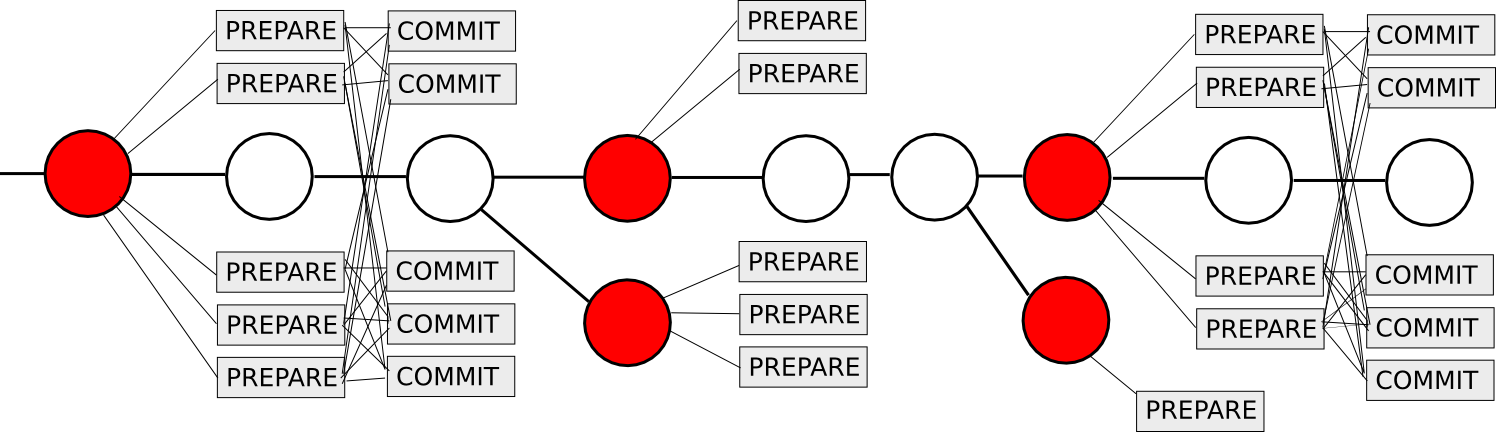
\includegraphics[width=5.5in]{prepares_commits.png}
\caption{Illustrating prepares, commits and checkpoints. Arrows represent \textit{dependency} (e.g. a commit depends on there being $\frac{2}{3}$ existing prepares)}
\label{fig:prepares_and_commits}
\end{figure}

During epoch $n$, validators are expected to send prepare and commit messages with $\epoch = n$ and $h$ equal to a checkpoint of epoch $n$. Prepare messages may specify as \hashsource a checkpoint for any previous epoch (preferably the preceding checkpoint) of \hash, and which is \textit{justified} (see below), and the \epochsource is expected to be the epoch of that checkpoint.

Validators only pay attention to prepares and commits if they have been included in blocks, even if those blocks are not part of the main chain. This simplifies our finalty mechanism because it allows it to be expressed as a fork choice rule where the ``score'' of a block only depends on the block and its children, putting it into a similar category as more traditional PoW-based fork choice rules such as the longest chain rule and GHOST\cite{sompolinsky2013accelerating}.

Unlike GHOST, however, this fork choice rule is also \textit{finality-bearing}: there exists a ``finality'' mechanism that has the property that (i) the fork choice rule always prefers finalized blocks over non-finalized competing blocks, and (ii) it is impossible for two incompatible checkpoints to be finalized unless at least $\frac{1}{3}$ of the validators violated one of the two Casper Commandments (a.k.a. slashing conditions):

\begin{enumerate}
   \item[\textbf{I.}] \textsc{A validator shalt not publish two or more nonidentical Prepares for same epoch.}
   
   In other words, a validator may Prepare at most exactly one (\hash, \epochsource, \hashsource) triplet for any given epoch \epoch.

   \item[\textbf{II.}] \textsc{A validator shalt not publish an Commit between the epochs of a Prepare statement.} 
    
   Equivalently, a validator may not publish

\begin{equation}
\langle \msgPREPARE, \epoch_p, \hash_p, \epochsource, \hashsource, \signature \rangle \hspace{0.5in} \textnormal{\textsc{and}} \hspace{0.5in} \langle \msgCOMMIT, \epoch_c, \hash_c, \signature \rangle \;, 
\label{eq:msgPREPARE}
\end{equation}

where the epochs satisfy $\epochsource < \epoch_c < \epoch_p$.

\end{enumerate}

If a validator violates a slashing condition, the evidence that they did this can be included into the blockchain as a transaction, at which point the validator's entire deposit will be taken away, with a 4\% ``finder's fee'' given to the submitter of the evidence transaction.

Earlier versions of Casper had four slashing conditions,\cite{minslashing} but we can reduce to two because of the requirements that (i) finalized hashes must be justified, and (ii) justified hashes must point to an already justified ancestor; these requirements ensure that blocks will not register commits or prepares that violate the other two slashing conditions, making them superfluous.

\section{Proofs of Safety and Plausible Liveness}
\label{sect:theorems}

We give a proof of two properties of Casper: \textit{accountable safety} and \textit{plausible liveness}. Accountable safety means that two conflicting checkpoints cannot be finalized unless $\geq \frac{1}{3}$ of validators violate a slashing condition (meaning at least one third of the total deposits are lost). Honest validators will never violate slashing conditions, so this implies the usual Byzantine fault tolerance safety property, but expressing this in terms of slashing conditions means that we are actually proving a stronger claim: if two conflicting checkpoints get finalized, then at least $\frac{1}{3}$ of validators were malicious, \textit{and we know whom to blame, and so we can maximally penalize them in order to make such faults expensive}.

Plausible liveness means that it is always possible for $\frac{2}{3}$ of honest validators to finalize a new checkpoint, regardless of what previous events took place.

\begin{figure}[h!tb]
\centering
    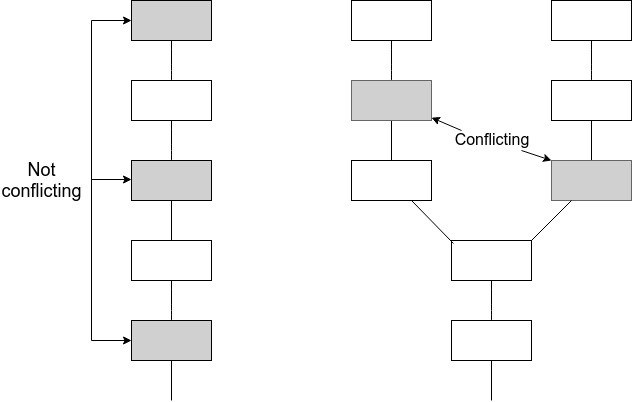
\includegraphics[width=5in]{conflicting_checkpoints.png}
\caption{Two checkpoints are \textit{conflicting} if they are on distinct chains, i.e. one is not an ancestor or a descendant of the other.}
\label{fig:conflicting_checkpoints}
\end{figure}


\begin{theorem}[Accountable Safety]
\label{theorem:safety}
Two conflicting checkpoints cannot be finalized unless $\geq \frac{1}{3}$ of validators violate a slashing condition.

\begin{proof}
Suppose the two conflicting checkpoints are $A$ in epoch $\epoch_A$ and $B$ in epoch $\epoch_B$. If both are finalized, this implies $\frac{2}{3}$ commits and $\frac{2}{3}$ prepares in epochs $\epoch_A$ and $e_B$. In the trivial case where $\epoch_A = \epoch_B$, this implies that some intersection of $\frac{1}{3}$ of validators must have violated slashing condition (1). In other cases, there must exist two chains $\Genesisblock < \ldots < \epoch_A^2 < \epoch_A^1 < \epoch_A$ and $\Genesisblock < \ldots < \epoch_B^2 < \epoch_B^1 < \epoch_B$ of justified checkpoints, both terminating at the genesis. Suppose without loss of generality that $\epoch_A > \epoch_B$. Then, there must be some $\epoch_A^i$ that either $\epoch_A^i = \epoch_B$ or $\epoch_A^i > \epoch_B > \epoch_A^{i+1}$. In the first case, since $A^i$ and $B$ both have $\frac{2}{3}$ prepares, at least $\frac{1}{3}$ of validators violated slashing condition (I). Otherwise, $B$ has $\frac{2}{3}$ commits and there exist $\frac{2}{3}$ prepares with $\epoch > B$ and $\epochsource < B$, so at least $\frac{1}{3}$ of validators violated slashing condition (II).
\end{proof}
\end{theorem}

\begin{theorem}[Plausible Liveness]
\label{theorem:liveness}
It is always possible for $\frac{2}{3}$ of honest validators to finalize a new checkpoint, regardless of what previous events took place.

\begin{proof}
Suppose that all existing validators have sent some sequence of prepare and commit messages. Let $M$ with epoch $\epoch_M$ be the highest-epoch checkpoint that was justified, and let $n \ge \epoch_M$ be the highest epoch in which an honest validator prepared. Honest validators have not committed on any block which is not justified. Hence, neither slashing condition stops them from making prepares on a descendant of $M$ in epoch $n+1$, using $\epoch_M$ as $\epochsource$, and then committing this child.
\end{proof}

\end{theorem}

\section{Fork Choice Rule}
\label{sect:forkchoice}

The mechanism described above ensures \textit{plausible liveness}; however, it by itself does not ensure \textit{actual liveness} - that is, while the mechanism cannot get stuck in the strict sense, it could still enter a scenario where the proposal mechanism (i.e. the proof of work chain) gets into a state where it never ends up creating a checkpoint that could get finalized.

In \figref{fig:forkchoice} we see one possible example.  In this case, $HASH1$ or any descendant thereof cannot be finalized without slashing $\frac{1}{6}$ of validators. However, miners on a proof of work chain would interpret $HASH1$ as the head and forever keep mining descendants of it, ignoring the chain based on $HASH0^\prime$ which actually could get finalized.

\begin{figure}[h!tb]
\centering
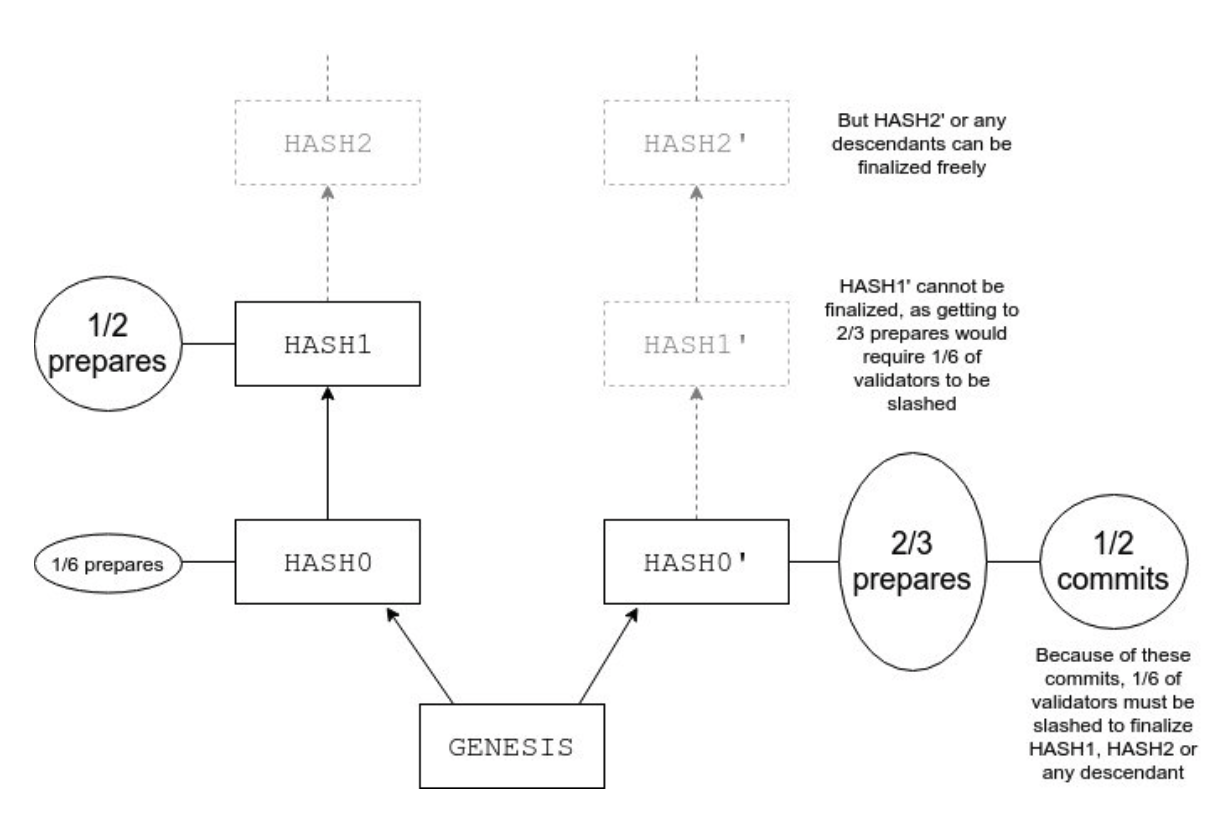
\includegraphics[width=5.5in]{fork4.png}
\caption{Miners following the traditional proof of work fork choice rule would create blocks on HASH1, but because of the slashing conditions only blocks on top of HASH1' can be finalized.}
\label{fig:forkchoice}
\end{figure}

In fact, when \textit{any} checkpoint gets $k > \frac{1}{3}$ commits, no conflicting checkpoint can get finalized without $k - \frac{1}{3}$ of validators getting slashed. This necessitates modifying the fork choice rule used by participants in the underlying proposal mechanism (as well as users and validators): instead of blindly following a longest-chain rule, there needs to be an overriding rule that (i) finalized checkpoints are favored, and (ii) when there are no further finalized checkpoints, checkpoints with more (justified) commits are favored.

One complete description of such a rule would be:

\begin{enumerate}
\item Start with HEAD equal to the genesis of the chain.
\item Select the descendant checkpoint of HEAD with the most commits (only justified checkpoints are admissible)
\item Repeat (2) until no descendant with commits exists.
\item Choose the longest proof of work chain from there.
\end{enumerate}

The commit-following part of this rule can be viewed as mirroring the ``greegy heaviest observed subtree'' (GHOST) rule that has been proposed for proof of work chains\cite{sompolinsky2013accelerating}. The symmetry is as follows. In GHOST, a node starts with the head at the genesis, then begins to move forward down the chain, and if it encounters a block with multiple children then it chooses the child that has the larger quantity of work built on top of it (including the child block itself and its descendants).

In this algorithm, we follow a similar approach, except we repeatedly seek the child that comes the closest to achieving finality. Commits on a descendant are implicitly commits on all of its lineage, and so if a given descendant of a given block has more commits than any other descendant, then we know that all children along the chain from the head to this descendant are closer to finality than any of their siblings; hence, looking for the \textit{descendant} with the most commits and not just the \textit{child} replicates the GHOST principle most faithfully. Finalizing a checkpoint requires $\frac{2}{3}$ commits within a \textit{single} epoch, and so we do not try to sum up commits across epochs and instead simply take the maximum.

This rule ensures that if there is a checkpoint such that no conflicting checkpoint can be finalized without at least some validators violating slashing conditions, then this is the checkpoint that will be viewed as the ``head'' and thus that validators will try to commit on.

\section{Allowing Dynamic Validator Sets}
\label{sect:join_and_leave}

The set of validators needs to be able to change.  New validators need to be able to join, and existing validators need to be able to leave.  To accomplish this, we define a variable kept track of in the state called the \textit{dynasty} counter. When a user sends a ``deposit'' transaction to become a validator, if this transaction is included in dynasty $n$, then the validator will be \textit{inducted} in dynasty $n+2$. The dynasty counter increments when the chain detects that the checkpoint of the current epoch that is part of its own history has been \textit{perfectly finalized} (that is, the checkpoint of epoch \epoch must be finalized during epoch \epoch, and the chain must learn about this before epoch \epoch ends). In simpler terms, when a user sends a ``deposit'' transaction, they need to wait for the transaction to be perfectly finalized, and then they need to wait again for the next epoch to be finalized; after this, they become part of the validator set. We call such a validator's \textit{start dynasty} $n+2$.

For a validator to leave, they must send a ``withdraw'' message. If their withdraw message gets included during dynasty $n$, the validator similarly leaves the validator set during dynasty $n+2$; we call $n+2$ their \textit{end dynasty}. When a validator withdraws, their deposit is locked for a long period of time (the \textit{withdrawal delay}, for now think ``four months'') before they can take their money out; if they are caught violating a slashing condition within that time then their deposit is forfeited.

For a checkpoint to be justified, it must be prepared by a set of validators which contains (i) at least $\frac{2}{3}$ of the current dynasty (that is, validators with $startDynasty \le curDynasty < endDynasty$), and (ii) at least $\frac{2}{3}$ of the previous dyansty (that is, validators with $startDynasty \le curDynasty - 1 < endDynasty$. Finalization with commits works similarly. The current and previous dynasties will usually greatly overlap; but in cases where they substantially diverge this ``stitching'' mechanism ensures that dynasty divergences do not lead to situations where a finality reversion or other failure can happen because different messages are signed by different validator sets and so equivocation is avoided.

\begin{figure}[h!tb]
\centering
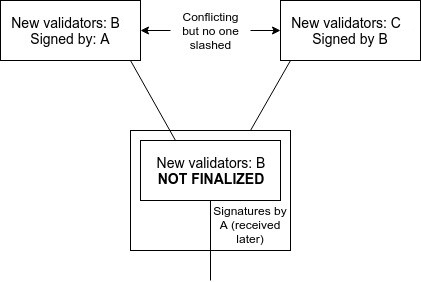
\includegraphics[width=4in]{validator_set_misalignment.png}
\caption{Without the validator set stitching mechanism, it's possible for two conflicting checkpoints to be finalized with no validators slashed}
\label{fig:dynamic}
\end{figure}

\subsection{Long Range Attacks}

Note that the withdrawal delay introduces a synchronicity assumption \textit{between validators and clients}. Because validators can withdraw their deposits after the withdrawal delay, there is an attack where a coalition of validators which had more than $\frac{2}{3}$ of deposits \textit{long ago in the past} withdraws their deposits, and then uses their historical deposits to finalize a new chain that conflicts with the original chain without fear of getting slashed.

\begin{figure}[h!tb]
\centering
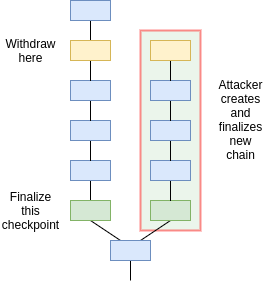
\includegraphics[width=3in]{LongRangeAttacks.png}
\caption{Despite violating slashing conditions to make a chain split, because the attacker has already withdrawn on both chains they do not lose any money. This is often called a \textit{long-range atack}.}
\label{fig:dynamic}
\end{figure}

We solve this problem by simply having clients not accept a finalized checkpoint that conflicts with finalized checkpoints that they already know about. Suppose that clients can be relied on to log on at least once every time $\delta$, and the withdrawal delay is $W$. Suppose an attacker sends one finalized checkpoint at time $0$, and then another right after. We pessimistically suppose the first checkpoint arrives at all clients at time $0$, and that the second reaches a client at time $\delta$. The client will then know of the fraud, and will be able to create and publish an evidence transaction. We then add a consensus rule that requires clients to reject chains that do not include evidence transactions that the client has known about for time $\delta$. Hence, clients will not accept a chain that has not included the evidence transaction within time $2 * \delta$. So if $W > 2 * \delta$ then slashing conditions are enforcible.

In practice, this means that if the withdrawal delay is four months, then clients will need to log on at least once per two months to avoid accepting bad chains for which attackers cannot be penalized.

\section{Recovering from Castastrophic Crashes}
\label{sect:leak}

Suppose that $>\frac{1}{3}$ of validators crash-fail at the same time---i.e, they are no longer connected to the network due to a network partition, computer failure, or are malicious actors. Then, no later checkpoint will be able to get finalized.

We can recover from this by instituting a ``leak'' which dissipates the deposits of validators that do not prepare or commit, until eventually their deposit sizes decrease low enough that the validators that \textit{are} preparing and committing are a $\frac{2}{3}$ supermajority. The simplest possible formula is something like ``validators with deposit size $D$ lose $D * p$ in every epoch in which they do not prepare and commit'', though to resolve catastrophic crashes more quickly a formula which increases the rate of dissipation in the event of a long streak of non-finalized blocks may be optimal.

The dissipated portion of deposits can either be burned or simply forcibly withdrawn and immediately refunded to the validator; which of the two strategies to use, or what combination, is an economic incentive concern and thus outside the scope of this paper.

Note that this does introduce the possibility of two conflicting checkpoints being finalized, with validators only losing money on one of the two checkpoints as seen in \figref{fig:commitsync}.

\begin{figure}[h!tb]
\centering
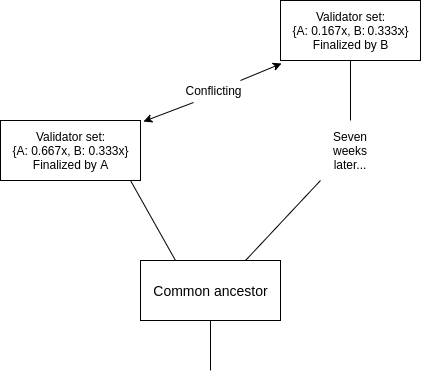
\includegraphics[width=4in]{CommitsSync.png}
\caption{The checkpoint on the left can be finalized immediately. The checkpoint on the right can be finalized after some time, once offline validator deposits sufficiently dissipate.}
\label{fig:commitsync}
\end{figure}

If the goal is simply to achieve maximally close to 50\% fault tolerance, then clients should simply favor the finalized checkpoint that they received earlier. However, if clients are also interested in defeating 51\% censorship attacks, then they may want to at least sometimes choose the minority chain. All forms of ``51\% attacks'' can thus be resolved fairly cleanly via ``user-activated soft forks'' that reject what would normally be the dominant chain. Particularly, note that finalizing even one block on the dominant chain precludes the attacking validators from preparing on the minority chain because of Commandment II, at least until their balances decrease to the point where the minority can commit, so such a fork would also serve the function of costing the majority attacker a very large portion of their deposits.

\section{Conclusions}

This introduces the basic workings of Casper the Friendly Finality Gadget's prepare and commit mechanism and fork choice rule, in the context of Byzantine fault tolerance analysis. Separate papers will serve the role of explaining and analyzing incentives inside of Casper, and the different ways that they can be parametrized and the consequences of these paramtrizations.

\section{Acknowledgements}

We thank Virgil Griffith for review and Sandro Lera for mathematics.


%\section{References}
\bibliographystyle{abbrv}
\bibliography{ethereum}

%\appendix
\clearpage
\part*{Appendix}

\section{Safety Failure}
\label{app:safetyfailure}
\todo{Put the full description/definition of conflicting blocks here.}




\section{Unused text}

\todo{This is where text goes that for which a home hasn't been found yet.  If no home is found, it will be deleted.}

Two other reasons to participate in stake pools are (i) to mitigate \emph{key theft risk} (i.e. an attacker hacking into their online machine and stealing the key), and (ii) to mitigate \emph{liveness risk}, the possibility that the validator node will go offline, perhaps because the operator does not have the time to manage a high-uptime setup.


\todo{Do we want to require that the Prepare be done in the first 1/2 of the epoch?  I'm mildly concerned there may not always be enough time to Commit.}

\todo{Remember: The only block you're allowed to Prepare is the last block of each epoch.}

\todo{Remember: Even if the Finalization goes through, the collective penalties are still applied.}


\textbf{Questions}
\begin{itemize}
\item It's unclear to me why we need $\epochsource$ in the Prepare.

\end{itemize}


%%%%%%%%%%%%%%%%%%%%%%%%%%%%%%%%%%%%%%%%%%%%%%%%%%%%%%


\end{document}
        
